 
\documentclass[12pt]{article}
%author 1: Andrew Schneider
%author 2: David Dobor
\usepackage[margin=1in]{geometry} 
\usepackage{amsmath,amsthm,amssymb}
 \usepackage{graphicx}
 \usepackage{multirow}
\usepackage[scaled]{helvet}
\usepackage{hyperref}
\usepackage[usenames,dvipsnames,svgnames,table]{xcolor}
\usepackage[T1]{fontenc}
\usepackage{palatino}
\usepackage{enumerate}
%\renewcommand*\familydefault{\sfdefault} %% Only if the base font of the document is to be sans serif

\newcommand{\N}{\mathbb{N}}
\newcommand{\Z}{\mathbb{Z}}


\newcommand{\blditA}{\textbf{\textit{A}}}
\newcommand{\blditB}{\textbf{\textit{B}}}
\newcommand{\blditC}{\textbf{\textit{C}}}
\newcommand{\blditP}{\textbf{\textit{P}}}
\newcommand{\blditQ}{\textbf{\textit{Q}}}
\newcommand{\bldI}{\textbf{I}}
\newcommand{\blditX}{\textbf{\textit{X}}}
 
\newenvironment{theorem}[2][Theorem]{\begin{trivlist}
\item[\hskip \labelsep {\bfseries #1}\hskip \labelsep {\bfseries #2.}]}{\end{trivlist}}
\newenvironment{lemma}[2][Lemma]{\begin{trivlist}
\item[\hskip \labelsep {\bfseries #1}\hskip \labelsep {\bfseries #2.}]}{\end{trivlist}}
\newenvironment{exercise}[2][Exercise]{\begin{trivlist}
\item[\hskip \labelsep {\bfseries #1}\hskip \labelsep {\bfseries #2.}]}{\end{trivlist}}
\newenvironment{problem}[2][Problem]{\begin{trivlist}
\item[\hskip \labelsep {\bfseries #1}\hskip \labelsep {\bfseries #2.}]}{\end{trivlist}}
\newenvironment{question}[2][Question]{\begin{trivlist}
\item[\hskip \labelsep {\bfseries #1}\hskip \labelsep {\bfseries #2.}]}{\end{trivlist}}
\newenvironment{answer}[2][Answer]{\begin{trivlist}
\item[\hskip \labelsep {\bfseries #1}\hskip \labelsep {\bfseries #2.}]}{\end{trivlist}}

\begin{document}
 \renewcommand{\arraystretch}{1.3}

 
\title{Stat 8003, Homework 4}%replace X with the appropriate number
\author{Group G: \ \ \texttt{sample( c( "David" , "Andrew",  "Salam" ))}
\\ %replace with your name
} %if necessary, replace with your course title
 
\maketitle
 
 %%%%%%%% Question 1 %%%%%%%%%
 \begin{question}{4.1} Suppose $X$ is a discrete random variables with $P(X = 1) = \theta$   and $ P(X = 2) = 1-\theta$. Three independent observations of $X$ are made: $x_1 = 1,\; x_2 = 2,\;  x_3 = 2$.
 \begin{enumerate}[(a)]
\item Find the method of moments estimate of $\theta$;
\item What is the likelihood function?
\item What is the MLE of $\theta$?:
\end{enumerate}
\end{question} 


  \textbf{\color{TealBlue}\emph{Answer:} } 
 $X$ is Bernoulli with parameter $\theta$:
  \[ 
X = 
  \begin{cases} 
       1    &  \text{with probability} \ \   \theta \\
       2  &  \text{with probability}  \ \ 1 - \theta \\
   \end{cases}
\]

We write its \texttt{pdf} compactly as:
$$
f(x \mid \theta) = \theta^{2 - x} (1 - \theta)^{x -1}
$$
(This function evaluates to $\theta $ when $X = 1$ and to $1 - \theta$ when $X = 2$. The likelihood function is the product of \texttt{pdf}s viewed as a function of $\theta$ for the observed data: $L(\theta; \tilde x) = \prod_i f(x_i \mid \theta) $. Here the data consist of three independent observations: $x_1 = 1, x_2 = 2, x_3 = 2$.)


 \begin{enumerate}[(a)] %@Andrew
\item The method of moments (MOM) estimate of $\theta$: 
\begin{equation*}
m_1 = E(X) = (1)(\theta) + (2)(1 - \theta) = \theta + 2 - 2\theta = 2 - \theta
\end{equation*}
So,
\begin{equation*}
\hat{\theta} = 2 - m_1
\end{equation*}
From our data, 
\begin{equation*}
m_1 = \bar{x} = \frac{1 + 2 + 2}{3} = \frac{5}{3}
\end{equation*}

so our method of moment estimate for $\hat{\theta}$ is 
\begin{equation*}
\hat{\theta} = 2 - \frac{5}{3} = \frac{1}{3}
\end{equation*}

\item The likelihood function for this data is:
\begin{align*}
L(\theta; x) &= \theta^{2 - 1} (1 - \theta)^{1 -1} \theta^{2 - 2} (1 - \theta)^{x -2}\theta^{2 - 2} (1 - \theta)^{x -2} \\
&= \theta (1 - \theta)^2
\end{align*}

\item To get the maximum likelihood estimate (MLE) for $\theta$, we can differentiate the likelihood function with respect to $\theta$, set it to zero, and solve for $\theta$. Alternatively, we can take the $\log$ of the likelihood function and set that to zero to solve for $\theta$:

\begin{align*}
\frac{d} {d \theta} \log (\theta (1 - \theta)^2) &= \frac{d} {d \theta} \left(\log \theta + 2 \log(1 - \theta) \right) = 0\\
\end{align*}
Or
\begin{align*}
\frac{1}{\theta} = \frac{2}{1 - \theta}\\
\end{align*}
\begin{align*}
1 - \theta = 2 \theta\\
\end{align*}
From where we get:
$$
\boxed{\hat \theta = \frac{1}{3}}
$$
\end{enumerate}

We now check whether this extremum is indeed a \emph{maximum}. We take the second derivative of $L(\theta; x)$, evaluate it at $\frac{1}{3}$ and see if it's negative. Indeed:
\begin{align*}
\frac{d^2} {d \theta^2} L(\theta; x) &= \frac{d} {d \theta} \left(\frac{1}{\theta} + \frac{2}{1 - \theta} \right) \\
&= -\frac{1}{\theta^2} + \frac{2}{(1 - \theta)^2} \\
&= -\frac{1}{(\frac{1}{3})^2} + \frac{2}{(1 - (\frac{1}{3}))^2} \\
&= -9 + \frac{9}{2}\\
&< 0 
\end{align*}
\begin{center}
So we indeed have a \emph{maximum} at  $\hat \theta = \frac{1}{3}$.
\end{center}

\bigskip
\bigskip
 %%%%%%%% Question 2 %%%%%%%%%
 \begin{question}{4.2} Consider an \texttt{i.i.d.} sample of random variables with density function
 $$
f(x \mid \sigma) = \frac{1}{2\sigma}exp(- \frac{|x|}{\sigma})
 $$
 \begin{enumerate}[(a)]
\item Find the MOM estimate of $\sigma$;
\item Find the MLE estimate of $\sigma$;
\end{enumerate}
\end{question} 


  \textbf{\color{TealBlue}\emph{Answer:} } 
 
  \begin{enumerate}[(a)]
\item \begin{equation*}
m_1 = E(X) = \int_{-\infty}^{+\infty}\frac{x}{2\sigma}exp(- \frac{|x|}{\sigma})dx $$\\$$
\end{equation*}
This is an integral of an \emph{odd} function, which should evaluate to zero:
\begin{align*}
      &= \int_{-\infty}^{0}\frac{x}{2\sigma}exp(- \frac{|x|}{\sigma})dx + \int_{0}^{+\infty}\frac{x}{2\sigma}exp(- \frac{|x|}{\sigma})dx \\
     &=-\int_{0}^{+\infty}\frac{x}{2\sigma}exp(- \frac{|x|}{\sigma})dx + \int_{0}^{+\infty}\frac{x}{2\sigma}exp(- \frac{|x|}{\sigma})dx \\
     & = 0
\end{align*}
This isn't any help to us. So let us consider $m_2$.
\begin{equation*}
m_2 = E(X^2) = \int_{-\infty}^{+\infty}\frac{x^2}{2\sigma}exp(- \frac{|x|}{\sigma})dx$$\\$$
    = 2\int_{0}^{+\infty}\frac{x^2}{2\sigma}exp(- \frac{x}{\sigma})dx$$\\$$
    = \frac{1}{\sigma}\int_{0}^{+\infty} x^2 exp(- \frac{x}{\sigma})dx
\end{equation*}
Substitute $(y = \frac{x}{\sigma})$
\begin{equation*}
    = \sigma^2\int_{0}^{+\infty} y^2 exp(-y)dy$$\\$$
\end{equation*}
We could recognize this as the Gamma function and write the result. 

Or continue:
\begin{equation*}
    = \sigma^2\bigg(-y^2e^{-y}\bigg|_0^{+\infty} + 2\int_{0}^{+\infty} y exp(-y)dy\bigg)$$\\$$
    = \sigma^2 \bigg( 0 + (-2ye^{-y})\bigg|_0^{+\infty} + 2\int_{0}^{+\infty} exp(-y)dy\bigg)$$\\$$
    = \sigma^2 \bigg( 0 + 0 - 2exp(-y)\bigg|_{0}^{+\infty}\bigg) = 2\sigma^2 
\end{equation*}
So $m_2 = 2\sigma^2$.

Therefore
 $$\boxed{\hat \sigma = \sqrt{\frac{m_2}{2}} }$$

\bigskip
\item The likelihood function is given by 
\begin{equation*}
L(\sigma;X) = \prod_{i=1}^n \frac{1}{2\sigma} exp(-\frac{|x_i|}{\sigma})
\end{equation*}
Taking the $log$ of this gives 
\begin{equation*}
l(\sigma;X) = -n\: log(2\sigma) + \sum_{i=1}^n \frac{-|x_i|}{\sigma}
\end{equation*}

Then taking the derivative with respect to $\sigma$ gives
\begin{equation*}
\frac{dl}{d\sigma} = -\frac{n}{\sigma} + \frac{1}{\sigma^2}\sum_{i=1}^n|x_i|
\end{equation*}
Setting this equal to zero we get
\begin{equation*}
\frac{n}{\sigma} = \frac{1}{\sigma^2}\sum_{i=1}^n|x_i|
\end{equation*}
i.e., 
\begin{equation*}
\boxed{\hat \sigma = \frac{1}{n}\sum_{i=1}^n|x_i|}
\end{equation*}

\end{enumerate}
 

\bigskip
\bigskip
 %%%%%%%% Question 3 %%%%%%%%%

\begin{question}{4.3} 
 In the shuttle example, let $X_i$ denote the number of damaged o-rings and $t_i$
the temperature, where $i = 1, 2, \dots, n$. Assume the model as
$$
\begin{cases} 
       X_i \mid p_i \sim \text{Binom}(2, p_i) \\
       p_i = \mathrm{e}^{(\beta_0 + \beta_1 t_i)} /  ( 1 +  {\mathrm{e}^{(\beta_0 + \beta_1 t_i)})}
\end{cases}
$$
\end{question}
 \begin{enumerate}[(a)]
\item Derive the log-likelihood function;

Since
\begin{align*}
f(x_i \mid p_i) &= {2 \choose x_i} \left(\frac{ exp(\beta_0 + \beta_1 t_i) } { 1 +  exp(\beta_0 + \beta_1 t_i)} \right)^{x_i}     \left( \frac{1} { ( 1 +  exp(\beta_0 + \beta_1 t_i) } \right)^{2 - x_i} \\
&=  {2 \choose x_i}  \frac{ exp(\beta_0 + \beta_1 t_i)^{x_i} } { (1 +  exp(\beta_0 + \beta_1 t_i) )^2} \\
\end{align*}

The likelihood is
\begin{align*}
L(\beta_0, \beta_1 ; \tilde x, \tilde t) &= \prod_{i=1}^n {2 \choose x_i} \frac{ exp(\beta_0 + \beta_1 t_i)^{x_i} } { (1 +  exp(\beta_0 + \beta_1 t_i) )^{2}} \\
\end{align*}

And thus the log likelihood is:
\begin{align*}
l(\beta_0, \beta_1  ; \tilde x, \tilde t) &= \log \prod_{i=1}^n {2 \choose x_i} +  \sum_{i=1}^n x_i (\beta_0 + \beta_1 t_i) - 2 \sum_{i=1}^n \log (1 + exp(\beta_0 + \beta_1 t_i) ) \\
&= Some \ Constant +  \beta_0 \sum_{i=1}^n x_i   + \beta_1 \sum_{i=1}^n x_i t_i - 2  \sum_{i=1}^n \log (1 + exp(\beta_0 + \beta_1 t_i) )
\end{align*}


\item  Set the equations for the maximum likelihood estimator of $\beta_0, \beta_1$
Since
\begin{align*}
    \begin{cases} 
         \frac {\partial l} {\partial \beta_0} = \sum_{i=1}^n x_i - 2 \sum_{i=1}^n \frac{ exp(\beta_0 + \beta_1 t_i) } {1 + exp(\beta_0 + \beta_1 t_i) }\\
         \frac {\partial l} {\partial \beta_1} = \sum_{i=1}^n x_i t_i - 2 \sum_{i=1}^n \frac{ t_i exp(\beta_0 + \beta_1 t_i) } {1 + exp(\beta_0 + \beta_1 t_i) }\\
    \end{cases}
\end{align*}
We set these partial derivatives to 0 and solve them for $\beta_0$ and $\beta_1$:
\begin{align*}
    \begin{cases} 
         \sum_{i=1}^n x_i - 2 \sum_{i=1}^n \frac{ exp(\beta_0 + \beta_1 t_i) } {1 + exp(\beta_0 + \beta_1 t_i) } = 0\\
         \sum_{i=1}^n x_i t_i - 2 \sum_{i=1}^n \frac{ t_i exp(\beta_0 + \beta_1 t_i) } {1 + exp(\beta_0 + \beta_1 t_i) } = 0\\
    \end{cases}
\end{align*}

\item  Derive the steps for the Newton-Raphson algorithm...

In previous equations, we denote the first one by $f_1(\beta_0, \beta_1)$, the second with $f_2(\beta_0, \beta_1)$ and then apply Newton-Raphson to following two-variable problem:
\begin{align*}
    \begin{cases} 
         f_1(\beta_0, \beta_1) = 0\\
         f_2(\beta_0, \beta_1) =  0\\
    \end{cases}
\end{align*}

The Jacobian matrix is:
\begin{align*}
J =
\left( {\begin{array}{*{20}c}
\frac{\partial f_1(\beta_0, \beta_1) }{\partial \beta_0}&\frac{\partial f_1(\beta_0, \beta_1) }{\partial \beta_1}\\
\frac{\partial f_2(\beta_0, \beta_1) }{\partial \beta_0}&\frac{\partial f_2(\beta_0, \beta_1) } {\partial \beta_1}\\
 \end{array} } \right) &=
\left( {\begin{array}{*{20}c}
 - 2 \frac{\partial  }{\partial \beta_0} \left(\sum_{i=1}^n \frac{ exp(\beta_0 + \beta_1 t_i) } {1 + exp(\beta_0 + \beta_1 t_i) } \right) & - 2 \frac{\partial }{\partial \beta_1} \left(\sum_{i=1}^n \frac{ exp(\beta_0 + \beta_1 t_i) } {1 + exp(\beta_0 + \beta_1 t_i) } \right) \\
- 2 \frac{\partial  }{\partial \beta_0} \left( \sum_{i=1}^n \frac{ t_i exp(\beta_0 + \beta_1 t_i) } {1 + exp(\beta_0 + \beta_1 t_i) } \right) & - 2 \frac{\partial  } {\partial \beta_1}  \left( \sum_{i=1}^n \frac{ t_i exp(\beta_0 + \beta_1 t_i) } {1 + exp(\beta_0 + \beta_1 t_i) } \right) \\
 \end{array} } \right)  \\ &= 
 \end{align*}
 %%%%%%%%%%%%%%%
 \begin{align*}
 = -2 \sum_i
\left( {\begin{array}{*{20}c}
\frac{ exp(\beta_0 + \beta_1 t_i) } {1 + exp(\beta_0 + \beta_1 t_i) } - \left(  \frac{ exp(\beta_0 + \beta_1 t_i) } {1 + exp(\beta_0 + \beta_1 t_i) }\right)^2    & t_i \left(\frac{ exp(\beta_0 + \beta_1 t_i) } {1 + exp(\beta_0 + \beta_1 t_i) } - \left(  \frac{ exp(\beta_0 + \beta_1 t_i) } {1 + exp(\beta_0 + \beta_1 t_i) }\right)^2\right)\\
t_i \left(\frac{ exp(\beta_0 + \beta_1 t_i) } {1 + exp(\beta_0 + \beta_1 t_i) } - \left(  \frac{ exp(\beta_0 + \beta_1 t_i) } {1 + exp(\beta_0 + \beta_1 t_i) }\right)^2\right) & t_i^2 \left(\frac{ exp(\beta_0 + \beta_1 t_i) } {1 + exp(\beta_0 + \beta_1 t_i) } - \left(  \frac{ exp(\beta_0 + \beta_1 t_i) } {1 + exp(\beta_0 + \beta_1 t_i) }\right)^2\right)\\
 \end{array} } \right)
\end{align*}

 %%%%%%%%%%
 \begin{align*}
 = -2 \sum_i
\left( {\begin{array}{*{20}c}
\frac{exp(\beta_0 + \beta_1 t_i) } { (1 + exp(\beta_0 + \beta_1 t_i))^2 } & t_i \frac{exp(\beta_0 + \beta_1 t_i) } { (1 + exp(\beta_0 + \beta_1 t_i))^2 }\\
t_i \frac{exp(\beta_0 + \beta_1 t_i) } { (1 + exp(\beta_0 + \beta_1 t_i))^2 } & t_i^2 \frac{exp(\beta_0 + \beta_1 t_i) } { (1 + exp(\beta_0 + \beta_1 t_i))^2 }\\
 \end{array} } \right)
\end{align*}


%%%%%%
%%%%%%
%%%%%%

We could invert this Jacobian and use the following Newton-Raphson update rule to find $\beta_0$ and $\beta_1$:
\begin{align*}
\left(
\begin{array}{c} 
   \beta_0^{i+1} \\
   \beta_1^{i+1}\\ 
\end{array}
\right)
=
\left(
\begin{array}{c} 
   \beta_0^{i} \\
   \beta_1^{i}\\ 
\end{array}
\right)
- J^{-1} 
\left(
\begin{array}{c} 
   f_1(\beta_0^{i}, \beta_1^{i} ) \\
   f_2(\beta_0^{i}, \beta_1^{i} ) \\
\end{array}
\right)
\end{align*} 

\bigskip
\bigskip
Before implementing this in \texttt{R}, and since these expressions look complicated, we try to simplify life for ourselves by making the following observations.

We can simplify the \texttt{R} implementation by noting that
the model given in this problem is equivalent to the following:
$$
\log\left(\frac{p_i}{1 - p_i}\right) = \beta_0 + \beta_1 t_i
$$
We will denote $\log\left(\frac{p_i}{1 - p_i}\right) = y_i$ and write
$$
y_i = \beta_0 + \beta_1 t_i
$$
Once we have estimates for  $\beta_0$ and $\beta_1$, we can then recover $p_i$ from $y_i$.

(We note that we could use \texttt{R}'s linear regression model to get the least squares estimates of $\beta_0$ and $\beta_1$. However, we will estimate these using Newton-Raphson instead.)

First,
\begin{align*}
L(\beta_0, \beta_1 ; \tilde t) &= \prod_{i=1}^n ( \beta_0 + \beta_1 t_i )\\
\end{align*}
and
\begin{align*}
l(\beta_0, \beta_1 ; \tilde t) &= \sum_{i=1}^n \log( \beta_0 + \beta_1 t_i )\\
\end{align*}

And we set the partial derivatives with respect to $\beta_0$ and $\beta_1$ to zero:
\begin{align*}
    \begin{cases} 
         \frac {\partial l} {\partial \beta_0} = \sum_{i=1}^n \frac{1} {\beta_0 + \beta_1 t_i} = 0\\
         \frac {\partial l} {\partial \beta_1} = \sum_{i=1}^n \frac{t_i} {\beta_0 + \beta_1 t_i} = 0\\
    \end{cases}
\end{align*}


We then apply Newton-Raphson to these guys.

\item Use the Newton-Raphson algorithm to calculate the maximum likelihood estimator of $\beta_0$ and $\beta_1$

The estimates for the parameters are:
\begin{align*}
\beta_0 = 9.0211846741774\\
\beta_1 = -0.154296115305373\\
\end{align*}

%then 



\item On January 28, 1986, the outside temperature was 31 degrees. Based on your estimated $\beta_0$ and $\beta_1$, what is the probability of an o-ring failure?

\begin{align*}
y &= 9.0211846741774-0.154296115305373  * 31 \\
\end{align*}

\begin{align*}
p = \frac{\mathrm{e}^y}{ 1 + {\mathrm{e}^y}}\\
\end{align*}
\begin{align*}
\boxed{p = 0.9857691}
\end{align*}


\item Based on your estimator, plot the probability $p$ against the temperature by letting temperature go from 30 degrees to 90 degrees.

The plot of the probability of failure for our estimates of $\beta$s looks like this:

\begin{center}
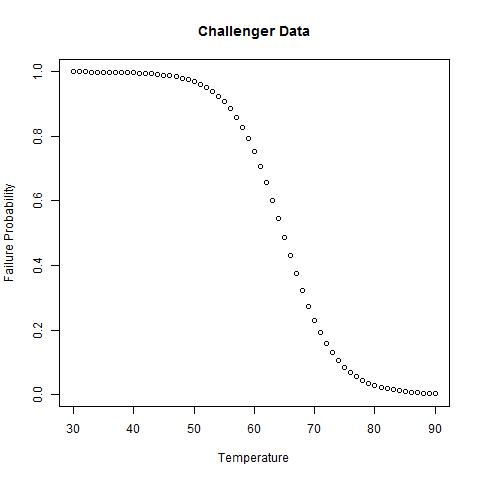
\includegraphics[width=10cm, height=10cm]{prob_vs_temp_plot_challenger}
\end{center}

\end{enumerate}

\end{document}
%%%%%%%%   ALTERNATIVE Part B, AND BEYOND %%%%%%%%%%%
%\bigskip
%\bigskip
%\bigskip
\bigskip
%\bigskip
%\bigskip
%\bigskip
%\bigskip
%\bigskip
%\bigskip
%\bigskip
%\bigskip
%\bigskip
%\bigskip
%\bigskip
%\bigskip
%
%WHAT FOLLOWS BELOW IS AN ALTERNATIVE TO THE ABOVE PARTS b) - f)
%\bigskip
%\bigskip
%\bigskip
%\bigskip
%\bigskip
%\bigskip
%
% \begin{enumerate}[(b)]
%\item We can simplify the formulas that follow, and their \texttt{R} implementation, if we note that
%the model given in this problem is equivalent to the following:
%$$
%\log\left(\frac{p_i}{1 - p_i}\right) = \beta_0 + \beta_1 t_i
%$$
%We will denote $\log\left(\frac{p_i}{1 - p_i}\right) = y_i$ and write
%$$
%y_i = \beta_0 + \beta_1 t_i
%$$
%Once we have estimates for  $\beta_0$ and $\beta_1$, we can then recover $p_i$ from $y_i$.
%
%(We note that we could use \texttt{R}'s linear regression model to get the least squares estimates of $\beta_0$ and $\beta_1$. However, we will estimate these using Newton-Raphson instead.)
%
%First,
%\begin{align*}
%L(\beta_0, \beta_1 ; \tilde t) &= \prod_{i=1}^n ( \beta_0 + \beta_1 t_i )\\
%\end{align*}
%and
%\begin{align*}
%l(\beta_0, \beta_1 ; \tilde t) &= \sum_{i=1}^n \log( \beta_0 + \beta_1 t_i )\\
%\end{align*}
%
%And we set the partial derivatives with respect to $\beta_0$ and $\beta_1$ to zero:
%\begin{align*}
%    \begin{cases} 
%         \frac {\partial l} {\partial \beta_0} = \sum_{i=1}^n \frac{1} {\beta_0 + \beta_1 t_i} = 0\\
%         \frac {\partial l} {\partial \beta_1} = \sum_{i=1}^n \frac{t_i} {\beta_0 + \beta_1 t_i} = 0\\
%    \end{cases}
%\end{align*}
%
%
%\item Now we apply Newton-Raphson to these guys.
%
%Denote the first one by $f_1(\beta_0, \beta_1)$, the second with $f_2(\beta_0, \beta_1)$ and then apply Newton-Raphson to following two-variable problem:
%\begin{align*}
%    \begin{cases} 
%         f_1(\beta_0, \beta_1) = 0\\
%         f_2(\beta_0, \beta_1) =  0\\
%    \end{cases}
%\end{align*}
%
%The Jacobian matrix is:
%\begin{align*}
%J &=
%\left( {\begin{array}{*{20}c}
%\frac{\partial f_1(\beta_0, \beta_1) }{\partial \beta_0}&\frac{\partial f_1(\beta_0, \beta_1) }{\partial \beta_1}\\
%\frac{\partial f_2(\beta_0, \beta_1) }{\partial \beta_0}&\frac{\partial f_2(\beta_0, \beta_1) } {\partial \beta_1}\\
% \end{array} } \right) \\
%&=
%\left( {\begin{array}{*{20}c}
%  - \sum_i \frac{1} {(\beta_0 + \beta_1 t_i)^2 } & -\sum_i \frac{t_i} {(\beta_0 + \beta_1 t_i)^2 }\\
%- \sum_i \frac{t_i} {(\beta_0 + \beta_1 t_i)^2 } & -\sum_i \frac{t_i^2} {(\beta_0 + \beta_1 t_i)^2 }\\
% \end{array} } \right)  \\
%\end{align*}
%
%
%\bigskip
%
%\item Let's suppose our estimates for the parameters are:
%\begin{align*}
%\beta_0 = 15.0429 \\
%\beta_1 = -0.2322 \\
%\end{align*}
%then 
%\begin{align*}
%y &= 15.0429 - 0.2322  * 31 = 7.8447 \\
%\end{align*}
%
%\begin{align*}
%p = \frac{\mathrm{e}^y}{ 1 + {\mathrm{e}^y}}\\
%\end{align*}
%\begin{align*}
%\boxed{p = 0.9996083}
%\end{align*}
%
%\item The plot of the probability of failure for our estimates of $\beta$s looks like this:
%
%\begin{center}
%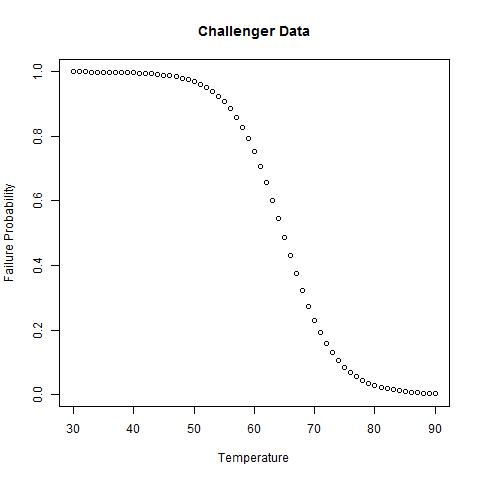
\includegraphics[width=10cm, height=10cm]{prob_vs_temp_plot_challenger}
%\end{center}
%
%\end{enumerate}
%



%We then take the inverse of the result. For shorthand, denoting $J$ as:
%\begin{align*}
%J=
%\left(
%\begin{array}{cl} 
%   a & b \\
%   c & d \\ 
%\end{array}
%\right)
%\end{align*} 
%Its inverse is
%\begin{align*}
%J^{-1} = \frac{1}{det(J)} 
%\left(
%\begin{array}{cc} 
%   d & -b \\
%   -c & a \\ 
%\end{array}
%\right)
%\end{align*} 


%%%%%%%%%%%%%% START STUFF ABOUT JACOBIAN NOT BEING ZERO %%%%%%%%%%%%%
%
%Now the determinant of this Jacobian is \emph{not} zero. Consider a small matrix with 2 obserbations, $t_1$ and $t_2$:
%\begin{align*}
%J &=
%\left( {\begin{array}{*{20}c}
%\frac{1 }{(\beta_0 + \beta1 t_1)^2} +\frac{1 }{(\beta_0 + \beta1 t_2)^2 }&\frac{t_1 }{(\beta_0 + \beta1 t_1)^2} +\frac{t_2}{(\beta_0 + \beta1 t_2)^2 }\\
%\frac{t_1 }{(\beta_0 + \beta1 t_1)^2} +\frac{t_2}{(\beta_0 + \beta1 t_2)^2 } &\frac{t_1^2 }{(\beta_0 + \beta1 t_1)^2} +\frac{t_2^2}{(\beta_0 + \beta1 t_2)^2 }\\
% \end{array} } \right) \\
%\end{align*}
%
%\begin{align*}
%det(J) &= \left( \frac{1 }{(\beta_0 + \beta_1 t_1)^2} +\frac{1 }{(\beta_0 + \beta_1 t_2)^2 } \right) 
%            \left( \frac{t_1^2 }{(\beta_0 + \beta_1 t_1)^2} +\frac{t_2^2 }{(\beta_0 + \beta_1 t_2)^2 } \right) \\
%       &- \left(\frac{t_1 }{(\beta_0 + \beta_1 t_1)^2} +\frac{t_2}{(\beta_0 + \beta_1 t_2)^2 }\right)
%            \left(\frac{t_1 }{(\beta_0 + \beta_1 t_1)^2} +\frac{t_2}{(\beta_0 + \beta_1 t_2)^2 }\right)\\
%        &= C_1^2 t_1^2 + C_1 C_2 t_2^2 + C_2 C_1 t_2^2  + C_2^2 t_2^2\\
%        &- C_1^2 t_1^2 + C_1 C_2 t_1 t_2 + C_2 C_1 t_2 t_1  + C_2^2 t_2^2\\
%        &\ne 0\\
%\end{align*}
%
%where 
%\begin{align*}
%C_1 = \frac{1 }{(\beta_0 + \beta_1 t_1)^2} \; \; \text{and} \; \; C_2 =  \frac{1 }{(\beta_0 + \beta_1 t_2)^2}
%\end{align*}
%
%
%%%%%%%%%%%%%% END STUFF ABOUT JACOBIAN NOT BEING ZERO %%%%%%%%%%%%%


